\documentclass[11pt,compress,t,notes=noshow, xcolor=table]{beamer}
\usepackage[]{graphicx}\usepackage[]{color}
% maxwidth is the original width if it is less than linewidth
% otherwise use linewidth (to make sure the graphics do not exceed the margin)
\makeatletter
\def\maxwidth{ %
  \ifdim\Gin@nat@width>\linewidth
    \linewidth
  \else
    \Gin@nat@width
  \fi
}
\makeatother

\definecolor{fgcolor}{rgb}{0.345, 0.345, 0.345}
\newcommand{\hlnum}[1]{\textcolor[rgb]{0.686,0.059,0.569}{#1}}%
\newcommand{\hlstr}[1]{\textcolor[rgb]{0.192,0.494,0.8}{#1}}%
\newcommand{\hlcom}[1]{\textcolor[rgb]{0.678,0.584,0.686}{\textit{#1}}}%
\newcommand{\hlopt}[1]{\textcolor[rgb]{0,0,0}{#1}}%
\newcommand{\hlstd}[1]{\textcolor[rgb]{0.345,0.345,0.345}{#1}}%
\newcommand{\hlkwa}[1]{\textcolor[rgb]{0.161,0.373,0.58}{\textbf{#1}}}%
\newcommand{\hlkwb}[1]{\textcolor[rgb]{0.69,0.353,0.396}{#1}}%
\newcommand{\hlkwc}[1]{\textcolor[rgb]{0.333,0.667,0.333}{#1}}%
\newcommand{\hlkwd}[1]{\textcolor[rgb]{0.737,0.353,0.396}{\textbf{#1}}}%
\let\hlipl\hlkwb

\usepackage{framed}
\makeatletter
\newenvironment{kframe}{%
 \def\at@end@of@kframe{}%
 \ifinner\ifhmode%
  \def\at@end@of@kframe{\end{minipage}}%
  \begin{minipage}{\columnwidth}%
 \fi\fi%
 \def\FrameCommand##1{\hskip\@totalleftmargin \hskip-\fboxsep
 \colorbox{shadecolor}{##1}\hskip-\fboxsep
     % There is no \\@totalrightmargin, so:
     \hskip-\linewidth \hskip-\@totalleftmargin \hskip\columnwidth}%
 \MakeFramed {\advance\hsize-\width
   \@totalleftmargin\z@ \linewidth\hsize
   \@setminipage}}%
 {\par\unskip\endMakeFramed%
 \at@end@of@kframe}
\makeatother

\definecolor{shadecolor}{rgb}{.97, .97, .97}
\definecolor{messagecolor}{rgb}{0, 0, 0}
\definecolor{warningcolor}{rgb}{1, 0, 1}
\definecolor{errorcolor}{rgb}{1, 0, 0}
\newenvironment{knitrout}{}{} % an empty environment to be redefined in TeX

\usepackage{alltt}
\newcommand{\SweaveOpts}[1]{}  % do not interfere with LaTeX
\newcommand{\SweaveInput}[1]{} % because they are not real TeX commands
\newcommand{\Sexpr}[1]{}       % will only be parsed by R
\newcommand{\xmark}{\ding{55}}%


\usepackage[english]{babel}
\usepackage[utf8]{inputenc}

\usepackage{dsfont}
\usepackage{verbatim}
\usepackage{amsmath}
\usepackage{amsfonts}
\usepackage{amssymb}
\usepackage{bm}
\usepackage{csquotes}
\usepackage{multirow}
\usepackage{longtable}
\usepackage{booktabs}
\usepackage{enumerate}
\usepackage[absolute,overlay]{textpos}
\usepackage{psfrag}
\usepackage{algorithm}
\usepackage{algpseudocode}
\usepackage{eqnarray}
\usepackage{arydshln}
\usepackage{tabularx}
\usepackage{placeins}
\usepackage{tikz}
\usepackage{setspace}
\usepackage{colortbl}
\usepackage{mathtools}
\usepackage{wrapfig}
\usepackage{bm}
\usepackage{amsmath}
\usepackage{pifont}
\usepackage{xcolor} %colored math symbols

\usetikzlibrary{shapes,arrows,automata,positioning,calc,chains,trees, shadows}
\tikzset{
  %Define standard arrow tip
  >=stealth',
  %Define style for boxes
  punkt/.style={
    rectangle,
    rounded corners,
    draw=black, very thick,
    text width=6.5em,
    minimum height=2em,
    text centered},
  % Define arrow style
  pil/.style={
    ->,
    thick,
    shorten <=2pt,
    shorten >=2pt,}
}

\usepackage{subfig}

% Defines macros and environments
\usepackage{../../style/lmu-lecture}


\let\code=\texttt
\let\proglang=\textsf

\setkeys{Gin}{width=0.9\textwidth}

\setbeamertemplate{frametitle}{\expandafter\uppercase\expandafter\insertframetitle}

\usepackage{bbm}
% basic latex stuff
\newcommand{\pkg}[1]{{\fontseries{b}\selectfont #1}} %fontstyle for R packages
\newcommand{\lz}{\vspace{0.5cm}} %vertical space
\newcommand{\dlz}{\vspace{1cm}} %double vertical space
\newcommand{\oneliner}[1] % Oneliner for important statements
{\begin{block}{}\begin{center}\begin{Large}#1\end{Large}\end{center}\end{block}}


%new environments
\newenvironment{vbframe}  %frame with breaks and verbatim
{
 \begin{frame}[containsverbatim,allowframebreaks]
}
{
\end{frame}
}

\newenvironment{vframe}  %frame with verbatim without breaks (to avoid numbering one slided frames)
{
 \begin{frame}[containsverbatim]
}
{
\end{frame}
}

\newenvironment{blocki}[1]   % itemize block
{
 \begin{block}{#1}\begin{itemize}
}
{
\end{itemize}\end{block}
}

\newenvironment{fragileframe}[2]{  %fragile frame with framebreaks
\begin{frame}[allowframebreaks, fragile, environment = fragileframe]
\frametitle{#1}
#2}
{\end{frame}}


\newcommand{\myframe}[2]{  %short for frame with framebreaks
\begin{frame}[allowframebreaks]
\frametitle{#1}
#2
\end{frame}}

\newcommand{\remark}[1]{
  \textbf{Remark:} #1
}


\newenvironment{deleteframe}
{
\begingroup
\usebackgroundtemplate{
\includegraphics[width=\paperwidth,height=\paperheight]{../style/color/red.png}}
 \begin{frame}
}
{
\end{frame}
\endgroup
}
\newenvironment{simplifyframe}
{
\begingroup
\usebackgroundtemplate{
\includegraphics[width=\paperwidth,height=\paperheight]{../style/color/yellow.png}}
 \begin{frame}
}
{
\end{frame}
\endgroup
}\newenvironment{draftframe}
{
\begingroup
\usebackgroundtemplate{
\includegraphics[width=\paperwidth,height=\paperheight]{../style/color/green.jpg}}
 \begin{frame}
}
{
\end{frame}
\endgroup
}
% https://tex.stackexchange.com/a/261480: textcolor that works in mathmode
\makeatletter
\renewcommand*{\@textcolor}[3]{%
  \protect\leavevmode
  \begingroup
    \color#1{#2}#3%
  \endgroup
}
\makeatother


\input{../../latex-math/basic-math}
\input{../../latex-math/basic-ml}
\input{../../latex-math/ml-nn}

\newcommand{\titlefigure}{figure/dropout_goals.png}
\newcommand{\learninggoals}{
  \item Recap: Ensemble Methods
  \item Dropout
  \item Augmentation
}

\title{Deep Learning}
\date{}

\begin{document}

\lecturechapter{Dropout and Augmentation}
\lecture{I2DL}

%%%%%%%%%%%%%%%%%%%%%%%%%%%%%%%%%%%%%%%%%%%%%%%%%%%%%%%%%%%%%%%%%%
%%%%%%%%%%%%%%%%%%%%%%%%%%%%%%%%%%%%%%%%%%%%%%%%%%%%%%%%%%%%%%%%%%
\section{Ensemble Methods}
\begin{vbframe}{Recap: Ensemble Methods}

\begin{itemize}
\item Idea: Train \textbf{several models} separately, and \textbf{average their prediction} (i.e.~perform \textbf{model averaging}).
%$$\frac{1}{k} \sum_{i=1}^k f_k(x|\theta)$$
\item Intuition: This improves performance on test set, since different models will not make the same errors.
\item Ensembles can be constructed in different ways, e.g.:
\begin{itemize}
\item by combining completely different kind of models (using different learning algorithms and loss functions).
\item by \textbf{bagging}: train the same model on $k$ datasets, constructed by sampling $n$ samples from original dataset.
\end{itemize}
\item Since training a neural network repeatedly on the same dataset results in different solutions (why?) it can even make sense to combine those.
\end{itemize}

\framebreak 

\begin{figure}
    \centering
      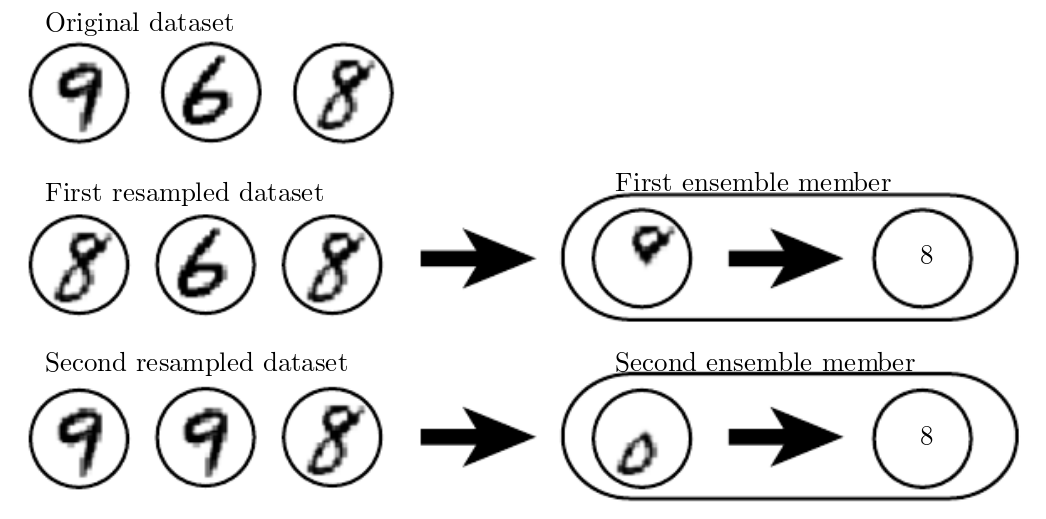
\includegraphics[width=11cm]{figure/bagging.png}
      \caption{ A cartoon description of bagging (Goodfellow et al. (2016))}
  \end{figure}

\end{vbframe}
%%%%%%%%%%%%%%%%%%%%%%%%%%%%%%%%%%%%%%%%%%%%%%%%%%%%%%%%%%%%%%%%%%
%%%%%%%%%%%%%%%%%%%%%%%%%%%%%%%%%%%%%%%%%%%%%%%%%%%%%%%%%%%%%%%%%%
\section{Dropout}

\begin{vbframe}{Dropout}
  \begin{itemize}
    \item %Dropout is a regularization technique for 
    Idea: reduce overfitting in neural networks by preventing complex co-adaptations of neurons.
    \item Method: during training, random subsets of the neurons are removed from the network (they are "dropped out").This is done by artificially setting the activations of those neurons to zero.
    \item Whether a given unit/neuron is dropped out or not is completely independent of the other units.
    \item If the network has $N$ (input/hidden) units, applying dropout to these units can result in $2^N$ possible 'subnetworks'.
    \item Because these subnetworks are derived from the same 'parent' network, many of the weights are shared.
    \item Dropout can be seen as a form of "model averaging".
  \end{itemize}
\framebreak
  \begin{figure}
    \centering
      \scalebox{0.8}{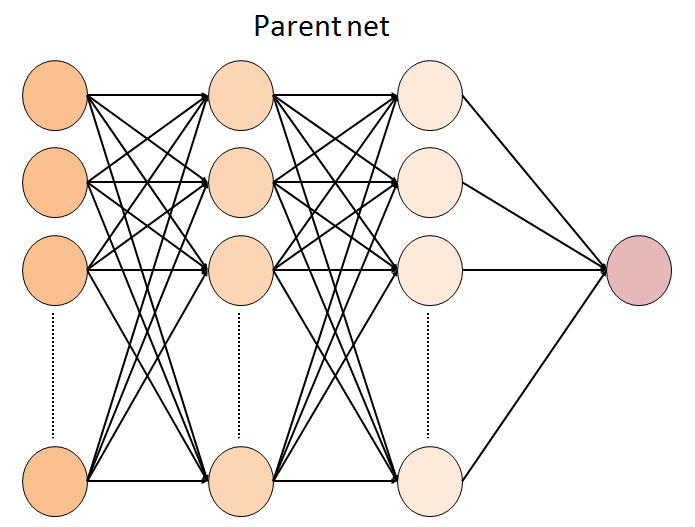
\includegraphics{figure/dropout.png}}
  \end{figure}
\framebreak
  \begin{figure}
    \centering
      \scalebox{0.8}{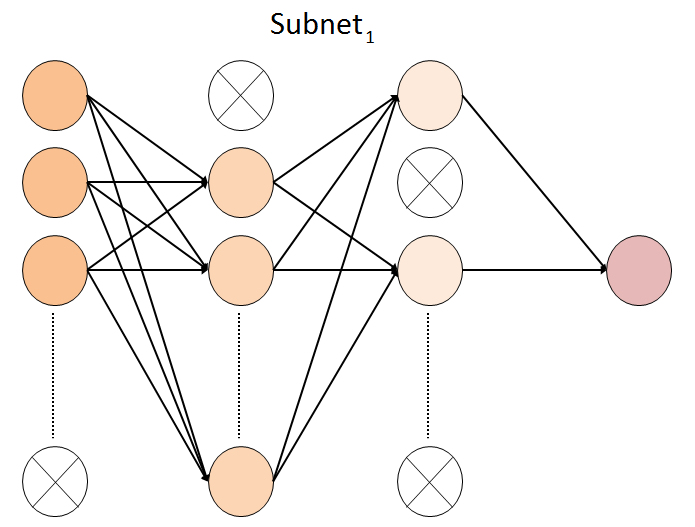
\includegraphics[width=10cm]{figure/subnet1.png}}
  \end{figure}
  In each iteration, for each training example (in the forward pass), a different (random) subset of neurons are dropped out.
\framebreak
  \begin{figure}
    \centering
      \scalebox{0.8}{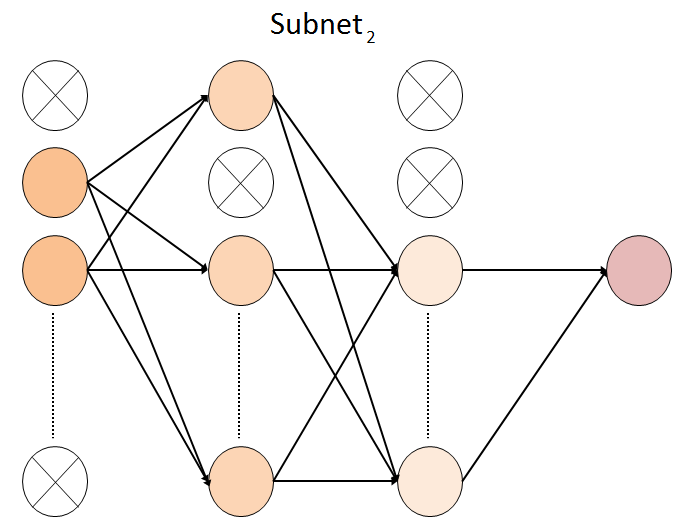
\includegraphics[width=10cm]{figure/subnet2.png}}
  \end{figure}
  In each iteration, for each training example (in the forward pass), a different (random) subset of neurons are dropped out.
\framebreak
  \begin{figure}
    \centering
      \scalebox{0.8}{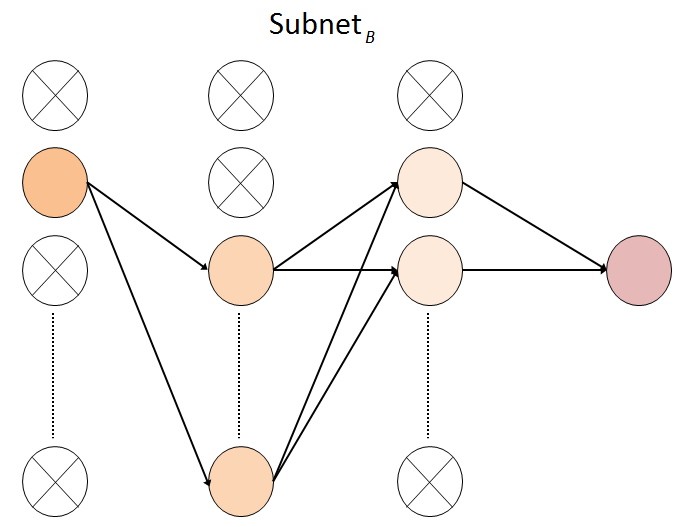
\includegraphics[width=10cm]{figure/subnet3.png}}
  \end{figure}
  In each iteration, for each training example (in the forward pass), a different (random) subset of neurons are dropped out.
\end{vbframe}


\begin{vbframe}{Dropout: Algorithm}
  \begin{itemize}
    \item To train with dropout a minibatch-based learning algorithm such as stochastic gradient descent is used.  
    \item For each training case in a minibatch, we randomly sample a binary vector/mask $\mu$ with one entry for each input or hidden unit in the network. The entries of $\mu$ are sampled independently from each other. 
    \item The probability of sampling a mask value of 0 (dropout) for one unit is a hyperparameter known as the 'dropout rate'. 
    \item A typical value for the dropout rate is $0.2$ for input units and $0.5$ for hidden units. 
    \item Each unit in the network is multiplied by the corresponding mask value resulting in a $subnet_{\mu}$. 
    \item Forward propagation, backpropagation, and the learning update are run as usual.
  \framebreak
  \begin{algorithm}[H]
  \footnotesize
  \caption{Training a (parent) neural network with dropout rate $p$}
    \begin{algorithmic}[1]
      \State Define parent network and initialize weights
      \For{each minibatch: }
        \For{each training sample: }
        \State Draw mask $\mu$ using $p$
        \State Compute forward pass for $subnet_{\mu}$
%        \State Compute the gradient of the loss for $network_{\mu}$
        \EndFor
        \State \parbox[t]{\dimexpr\linewidth-\algorithmicindent}{Update the weights of the (parent) network by performing a gradient descent step with weight decay}
      \EndFor
    \end{algorithmic}
  \end{algorithm}
    \item The derivatives wrt. each parameter are averaged over the training cases in each mini-batch. Any training case which does not use a parameter contributes a gradient of zero for that parameter.
      \end{itemize}
\end{vbframe}

\begin{vbframe}{Dropout: Weight scaling}
  \begin{itemize}
    \item The weights of the network will be larger than normal because of dropout. Therefore, to obtain a prediction at test time the weights must be first scaled by the chosen dropout rate.
    \item This means that if a unit (neuron) is retrained with probability $p$ during training, the weight at test time of that unit is multiplied by $p$.
  \begin{figure}
      \centering
    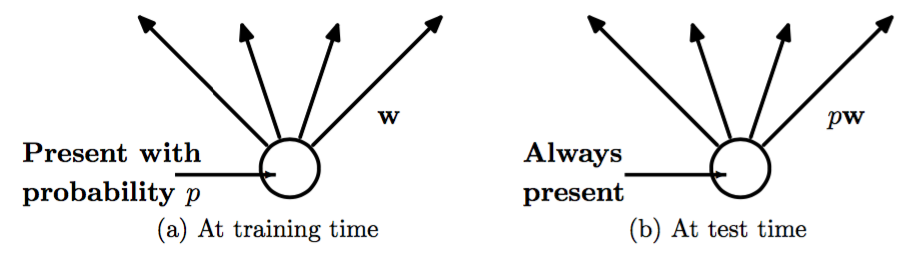
\includegraphics[width=7cm]{figure/dropout_neuron.png}
    \tiny{\\ Credit: Srivastava et. al. (2014)}
  \end{figure}
  \item Weight scaling ensures that the expected total input to a neuron/unit at test time is roughly the same as the expected total input to that unit at train time, even though many of the units at train time were missing on average
  \item Rescaling of the weights can also be performed at training time instead, after each weight update at the end of the mini-batch. This is sometimes called 'inverse dropout'. Keras and PyTorch deep learning libraries implement dropout in this way.
 % \item Weight scaling ensures that for any hidden unit the \textbf{expected} output (under the distribution used to drop units at training time) is the same as the \textbf{actual} output at test time. 
  \end{itemize}
\end{vbframe}

%%%%%%%%%%%%%%%%%%%%%%%%%%%%%%%%%%%%%%%%%%%%%%%%%%%%%%%%%
\begin{vbframe}{Dropout: Example}
\begin{minipage}{0.5\textwidth}
  \begin{itemize}
    \item To demonstrate how dropout can easily improve generalization we compute neural networks with the structure showed on the right.
    \item Each neural network we fit has different dropout probabilities, a tuple where one probability is for the input layer and one is for the hidden layers. We consider the tuples $(0;0) , (0.2;0.2) \text{ and } (0.6;0.5)$.
  \end{itemize}
  \end{minipage}
  \begin{minipage}{0.45\textwidth}
  \begin{figure}
    \centering
    \vspace{-0.5cm}
      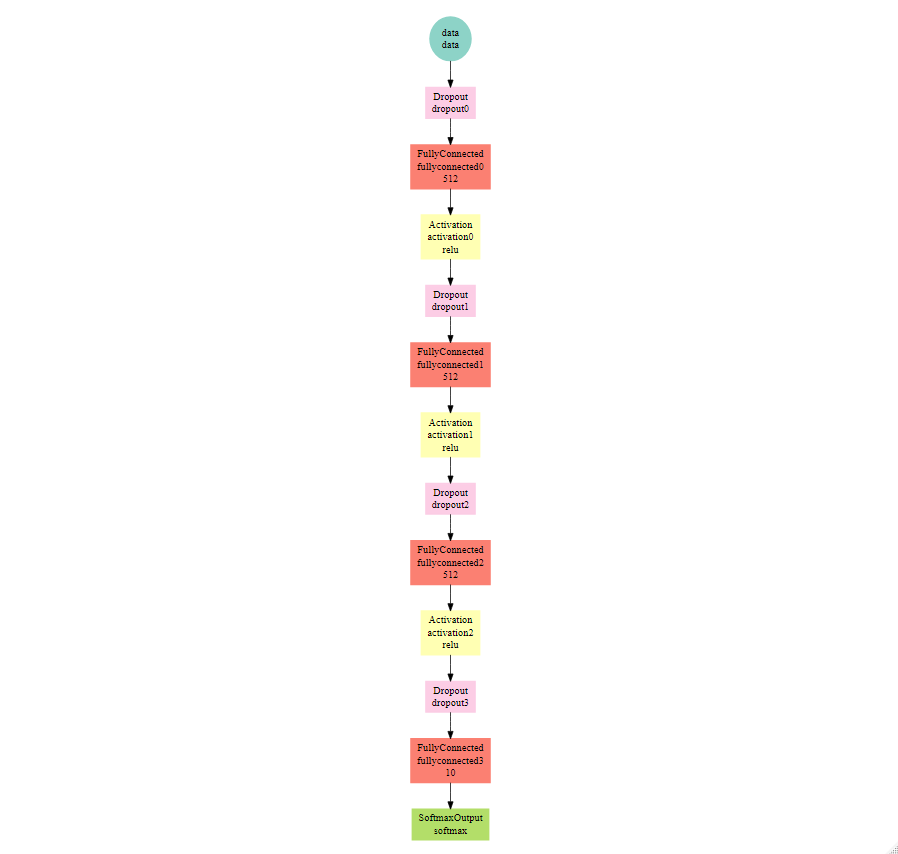
\includegraphics[width=9cm]{figure/mxnet_graph_dropout.png}
  \end{figure}
  \end{minipage}
\framebreak
%
%\begin{knitrout}\scriptsize
%\definecolor{shadecolor}{rgb}{0.969, 0.969, 0.969}\color{fgcolor}
%
%{\centering 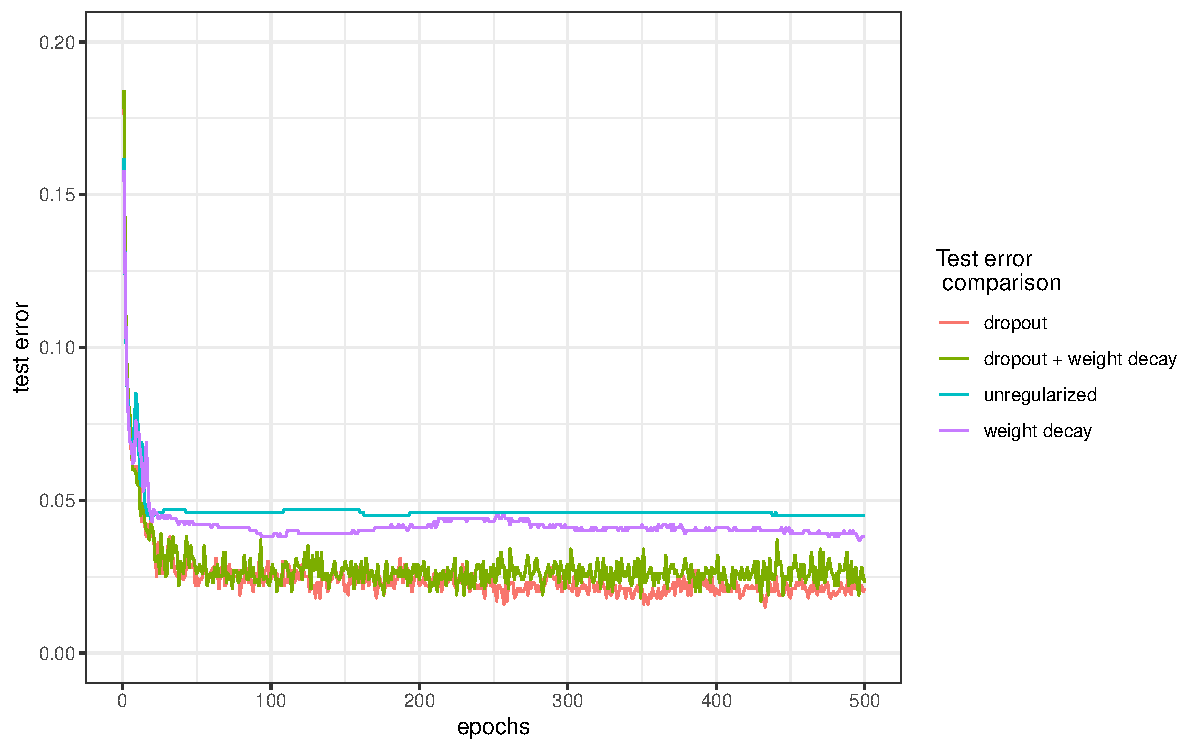
\includegraphics[width=0.95\textwidth]{figure/unnamed-chunk-3-1} 
%
%}
%
%
%\end{knitrout}
%Higher dropout rates lead to higher training error. 
%\framebreak

\begin{knitrout}\scriptsize
\definecolor{shadecolor}{rgb}{0.969, 0.969, 0.969}\color{fgcolor}

{\centering 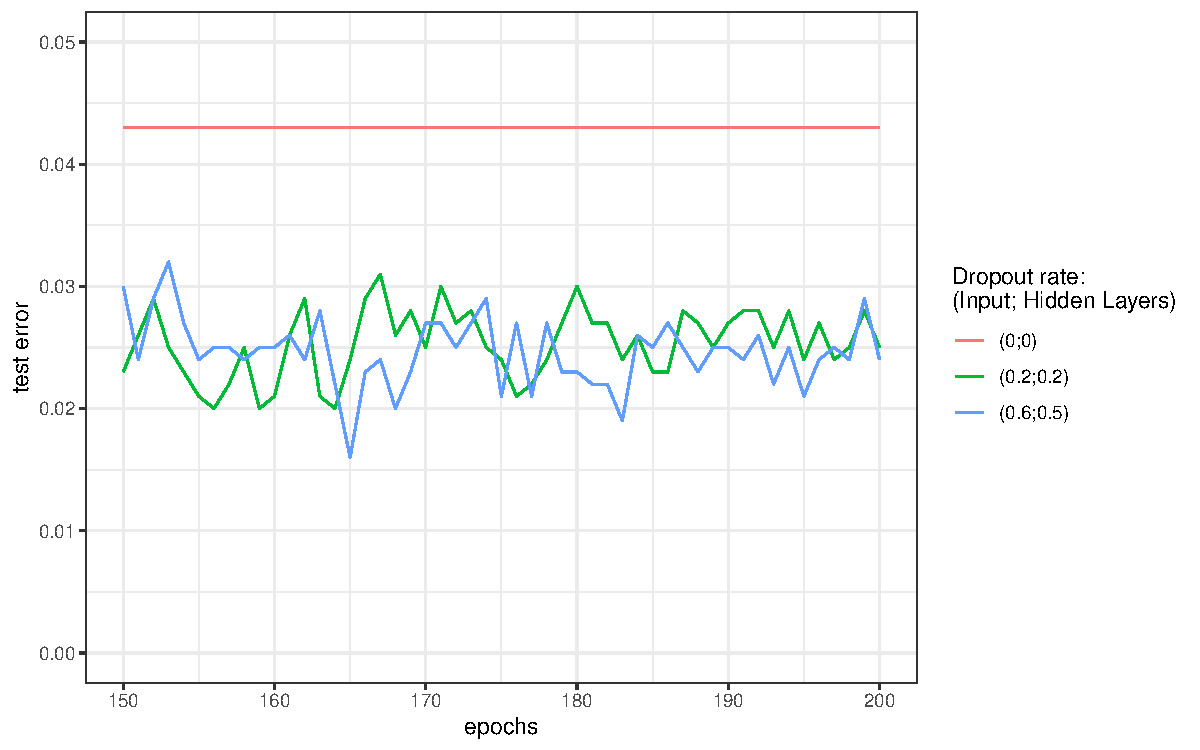
\includegraphics[width=0.95\textwidth]{figure/unnamed-chunk-4-1} 

}


\end{knitrout}
Dropout rate of 0 (no dropouts) leads to higher test error than dropping some units out. 
\end{vbframe}
%%%%%%%%%%%%%%%%%%%%%%%%%%%%%%%%%%%%%%%%%%%%%%%%%%%%%%%%%%%%%%%%%%
%%%%%%%%%%%%%%%%%%%%%%%%%%%%%%%%%%%%%%%%%%%%%%%%%%%%%%%%%%%%%%%%%%
\begin{vbframe}{Dropout, weight decay or both?}

\begin{knitrout}\scriptsize
\definecolor{shadecolor}{rgb}{0.969, 0.969, 0.969}\color{fgcolor}

{\centering 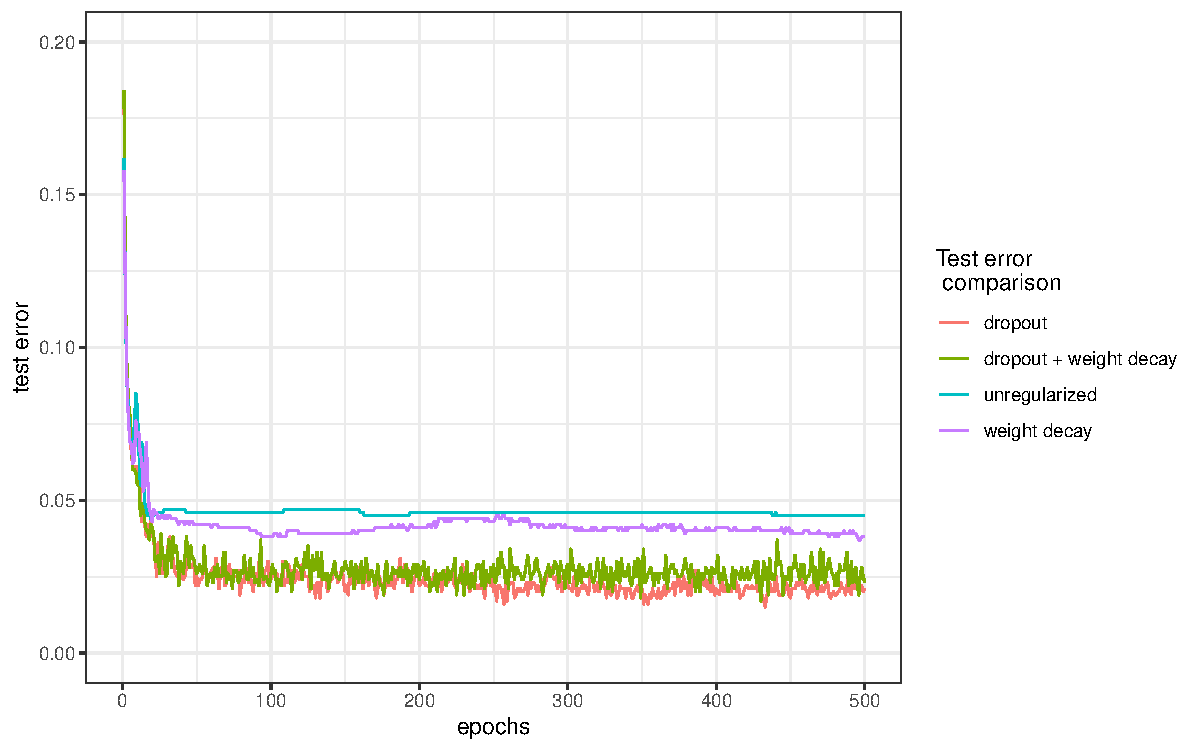
\includegraphics[width=0.95\textwidth]{figure/unnamed-chunk-5-1} 

}


\end{knitrout}
Here, dropout leads to a smaller test error than using no regularization or solely weight decay. 
\end{vbframe}
%%%%%%%%%%%%%%%%%%%%%%%%%%%%%%%%%%%%%%%%%%%%%%%%%%%%%%%%%%%%%%%%%%
%%%%%%%%%%%%%%%%%%%%%%%%%%%%%%%%%%%%%%%%%%%%%%%%%%%%%%%%%%%%%%%%%%

\section{Dataset Augmentation}
\begin{vbframe}{Dataset Augmentation}
  \begin{itemize}
    \item Problem: low generalization because high ratio of $$\frac{\text{complexity of the model}}{\text{\#train data}}$$
    \item Idea: artificially increase the train data.
      \begin{itemize}
        \item Limited data supply $\rightarrow$ create \enquote{fake data}! 
      \end{itemize}
    \item Increase variation in inputs \textbf{without} changing the labels.
    \item Application:
      \begin{itemize}
        \item Image and Object recognition (rotation, scaling, pixel translation, flipping, noise injection, vignetting, color casting, lens distortion, injection of random negatives)
        \item Speech recognition (speed augmentation, vocal tract perturbation)
      \end{itemize}
  \end{itemize}
\framebreak
  \begin{figure}
    \centering
      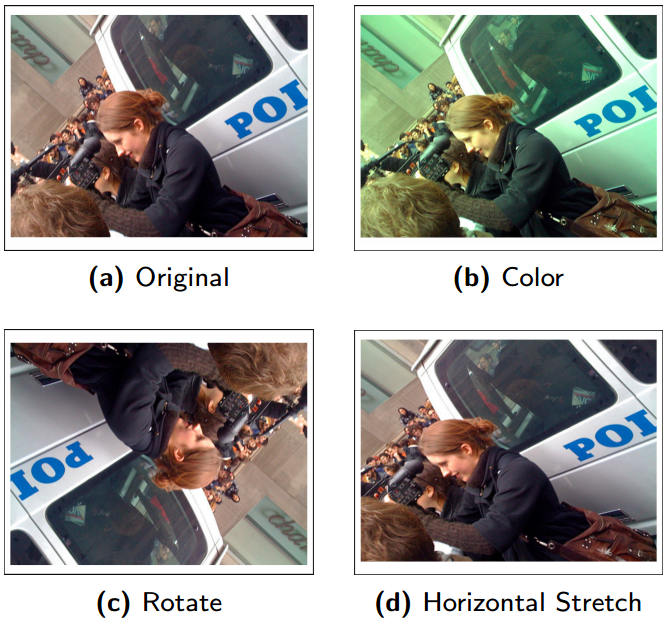
\includegraphics[width=7cm]{figure/data_augmentation_1.png}
      \caption{(Wu et al. (2015))}
  \end{figure}
\framebreak
  \begin{figure}
    \centering
      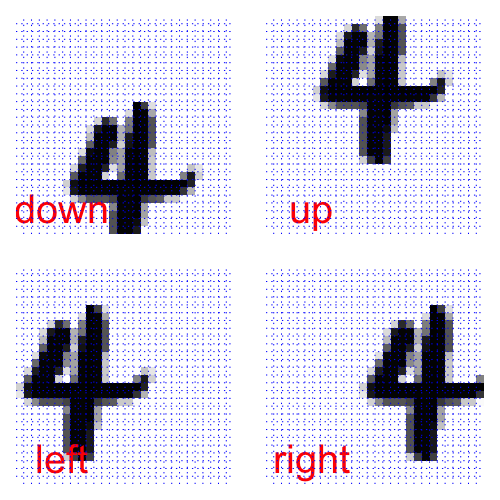
\includegraphics[width=6cm]{figure/data_augmentation_2.png}
      \caption{(Wu et al. (2015))}
  \end{figure}
  $\Rightarrow$ careful when rotating digits (6 will become 9 and vice versa)!
\end{vbframe}
%%%%%%%%%%%%%%%%%%%%%%%%%%%%%%%%%%%%%%%%%%%%%%%%%%%%%%%%%%%%%%%%%%
%%%%%%%%%%%%%%%%%%%%%%%%%%%%%%%%%%%%%%%%%%%%%%%%%%%%%%%%%%%%%%%%%%
%\section{Noise Robustness}
%\begin{vbframe}{Artificial Noise}
%Idea: Intentionally inject noise to the model, e.g.~inject noise 
%  \begin{itemize} 
%    \item  \textbf{to the input} to make the model more robust to small variations.
%  %  \item This method may force the model to \enquote{grow} weights in regions of flat minima. Thus, the noisy model may not find perfect minima but its approximations lie in a flatter surrounding.
%   (Bishop (1995) shows that for some models this has the same effect as parameter norm penalization.)
%   \item \textbf{to the weights}, which can interpreted as stochastic implementation of Bayesian inference and pushes the model to flat minima in parameter space. 
%    \item \textbf{to the outputs}  to account for possible errors in the labeling process. E.g.,~for \textbf{label smoothing} one replaces the label $1$ of a correct class by $1-\epsilon$ and the label $0$ of the $g$ remaining by $\frac{\epsilon}{g-1}$.
%    %In practice, it is common to apply noise to the outputs. This strategy is termed label smoothing as it incorporates a small noise term on the labels of the classification outputs. The intuition is to account for possible errors in the labeling process.
%  \end{itemize}
%\end{vbframe}
%


%%%%%%%%%%%%%%%%%%%%%%%%%%%%%%%%%%%%%%%%%%%%%%%%%%%%%%%%%%%%%%%%%%

%%%%%%%%%%%%%%%%%%%%%%%%%%%%%%%%%%%%%%%%%%%%%%%%%%%%%%%%%%%%%%%%%%
%%%%%%%%%%%%%%%%%%          REFERENCES          %%%%%%%%%%%%%%%%%%
%%%%%%%%%%%%%%%%%%%%%%%%%%%%%%%%%%%%%%%%%%%%%%%%%%%%%%%%%%%%%%%%%%
\begin{vbframe}
\frametitle{References}
\footnotesize{
\begin{thebibliography}{99}
%%%%%%%%%%%%%%%%%%%%%%%%%%%%%%%%%%
\bibitem[Ian Goodfellow et al., 2016]{1} Ian Goodfellow, Yoshua Bengio and Aaron Courville (2016)
\newblock Deep Learning
\newblock \emph{\url{http://www.deeplearningbook.org/}}
%%%%%%%%%%%%%%%%%%%%%%%%%%%%%%%%%%
\bibitem[Hinton et al., 2012]{2} Geoffrey E Hinton, Nitish Srivastava, Alex Krizhevsky Ilya Sutskever and Ruslan Salakhutdinov (2012)
\newblock Improving neural networks by preventing co-adaptation of feature detectors
\newblock \emph{\url{http://arxiv.org/abs/1207.0580}}
%%%%%%%%%%%%%%%%%%%%%%%%%%%%%%%%%%
    \bibitem[Srivastava et. al., 2014]{3} Nitish Srivastava, Geoffrey Hinton, Alex Krizhevsky Ilya Sutskever and Ruslan Salakhutdinov (2012)
  \newblock Dropout:  A Simple Way to Prevent Neural Networks from Overfitting
  \newblock \emph{\url{http://jmlr.org/papers/v15/srivastava14a.html}}
%   %%%%%%%%%%%%%%%%%%%%%%%%%%%%%%%%%%
\bibitem[Wu et al., 2015]{4} Wu Ren, Yan Shengen, Shan Yi, Dang Qingqing and Sun Gang (2015)
\newblock Deep Image: Scaling up Image Recognition
\newblock \emph{\url{https://arxiv.org/abs/1501.02876}}
%   %%%%%%%%%%%%%%%%%%%%%%%%%%%%%%%%%%
%\bibitem[Bishop, Chris M., 1995]{5} Bishop, Chris M. (1995)
%\newblock Training with Noise is Equivalent to Tikhonov Regularization
%\newblock \emph{\url{https://www.microsoft.com/en-us/research/wp-content/uploads/2016/02/bishop-tikhonov-nc-95.pdf}}


\end{thebibliography}
}
\end{vbframe}
%%%%%%%%%%%%%%%%%%%%%%%%%%%%%%%%%%%%%%%%%%%%%%%%%%%%%%%%%%%%%%%%%%
%%%%%%%%%%%%%%%%%%%%%%%%%%%%%%%%%%%%%%%%%%%%%%%%%%%%%%%%%%%%%%%%%%

\endlecture
\end{document}
